\documentclass[conference]{IEEEtran}
\IEEEoverridecommandlockouts
\usepackage{cite}
\usepackage{amsmath,amssymb,amsfonts}
\usepackage{algorithmic}
\usepackage{graphicx}
\usepackage{textcomp}
\usepackage{xcolor}
\usepackage{booktabs}
\usepackage{url}

\def\BibTeX{{\rm B\kern-.05em{\sc i\kern-.025em b}\kern-.08em
    T\kern-.1667em\lower.7ex\hbox{E}\kern-.125emX}}

\begin{document}

\title{Who Connects the Departments?\\Dependence and Resilience in the SNAP email-Eu-core Network}

\author{
\IEEEauthorblockN{Jiening Yang}
\IEEEauthorblockA{\textit{Department of Electrical and Computer Engineering} \\
\textit{Carnegie Mellon University}\\
Pittsburgh, PA, USA \\
jieningy@andrew.cmu.edu}
\and
\IEEEauthorblockN{Yikang Cheng}
\IEEEauthorblockA{\textit{Department of Electrical and Computer Engineering} \\
\textit{Carnegie Mellon University}\\
Pittsburgh, PA, USA \\
yikangc@andrew.cmu.edu}
}

\maketitle

\begin{abstract}
We investigate organizational dependence and network resilience in the SNAP email-Eu-core communication network of 1,005 employees across 42 departments. We formalize direct department-pair dependence and contrast degree-based cross-department contacts with shortest-path directed betweenness. Targeted node removal reveals that deleting high-contact employees severely degrades cross-department edge connectivity, whereas betweenness-targeted deletion causes greater loss in directed reachability. Our findings highlight structural vulnerabilities and provide a baseline for resilience-enhancing interventions.
\end{abstract}

\begin{IEEEkeywords}
complex networks, organizational communication, network resilience, node removal, betweenness centrality
\end{IEEEkeywords}

\section{Introduction and Motivation}
In large modern institutions, inter-departmental collaboration is essential for innovation and operational continuity. While aggregate communication networks often appear densely interconnected, actual cross-department coordination frequently hinges on a handful of boundary-spanning individuals. In organizational science, such individuals act as information bridges; however, in network theory, they represent potential single points of structural failure. If key boundary personnel leave, become unavailable, or experience burnout, inter-departmental information channels can become severely degraded or severed.

This project investigates the concentration of cross-department contacts and the structural resilience of communication pathways within a large European research institution using the SNAP \textit{email-Eu-core} dataset \cite{snap-email}. We examine two central questions:
\begin{enumerate}
    \item To what extent does direct communication between departmental pairs depend on specific individual employees?
    \item How does targeted removal of key personnel—ranked either by direct cross-department contact volume or by global directed path brokerage—impact network edge retention and cross-department directed reachability compared to random employee turnover?
\end{enumerate}

To answer these questions, our approach combines granular structural analysis of ordered department-pair relationships with controlled node-removal experiments. By mapping pairwise departmental dependencies and contrasting local contact degree against global shortest-path betweenness centrality, we identify critical institutional bottlenecks. We then rigorously simulate employee departures under equal budget constraints, quantifying structural degradation via exact path reachability.

\section{Previous Work}
Our study builds upon and connects three distinct threads in network science and organizational analysis:

\textbf{Higher-order structures and organizational clustering:} Yin et al. \cite{yin2017local} developed local higher-order graph clustering techniques grounded in network motifs, demonstrating that directional subgraphs reveal core functional organization in complex systems. Their analysis utilized the SNAP email-Eu-core dataset as a primary benchmark. While their focus was on unsupervised community discovery, our work takes advantage of the provided ground-truth institutional department labels to evaluate dependencies between predefined functional units.

\textbf{Path brokerage and betweenness centrality:} Brandes \cite{brandes2001faster} introduced an $O(NM)$ algorithm for computing shortest-path betweenness centrality on directed networks, enabling the exact identification of path-brokerage roles without heuristic approximations. In this work, we compute exact directed betweenness across all 1,005 employees using the NetworkX implementation \cite{networkx-betweenness}. We compare this path-based brokerage metric against a simpler, local measure of cross-departmental contact degree, demonstrating that path mediation and direct contact volume capture distinct organizational roles.

\textbf{Network resilience and targeted node removal:} The foundational work of Albert, Jeong, and Barab{\'a}si \cite{albert2000error} demonstrated that scale-free topologies exhibit robust tolerance against random failure but acute fragility under targeted attack on high-degree hubs. We extend this classic paradigm to an empirical institutional communication graph with explicit multi-department partition. Rather than merely assessing giant component fragmentation, we introduce exact cross-department pairwise reachability via strongly connected component (SCC) DAG condensation, providing an accurate, semantics-aware measure of organizational communication continuity.

\section{Approach}

\subsection{Dataset and Network Construction}
We analyze the SNAP \textit{email-Eu-core} benchmark dataset \cite{snap-email}, which records internal email exchanges at a major European research institute over an 18-month duration. Each directed edge $(u, v)$ indicates that employee $u$ sent at least one email to employee $v$. The original dataset contains $1,005$ employees partitioned into $42$ disjoint, anonymous departments, comprising $25,571$ unique directed edges. Department sizes range from $1$ to $109$ employees (median $17.5$).

We construct an unweighted, directed graph $G = (V, E)$. Network validation ensures all edge endpoints have valid department labels and eliminates self-loops ($(u, u)$), as self-communication does not represent organizational interaction. Removing 642 self-loops leaves $|E| = 24,929$ valid directed edges, partitioned into $16,284$ cross-department edges (65.3\%) and $8,645$ internal edges (34.7\%). All $1,005$ employees are preserved, including 19 isolated nodes resulting from self-loop elimination. The largest weakly connected component (WCC) contains $986$ nodes, and the largest strongly connected component (SCC) contains $803$ nodes.

\subsection{Research Questions and Mathematical Formulation}
We formulate our inquiry through three concrete research questions:

\textbf{RQ1: Concentration of Department-Pair Contacts.} For any two distinct departments $A$ and $B$, let $E_{AB} \subseteq E$ denote the set of directed edges directed from employees in $A$ to employees in $B$. For each employee $v \in A \cup B$, let $c_{AB}(v)$ denote the number of edges in $E_{AB}$ incident to $v$. For pairs with $|E_{AB}| \ge 1$, we define the directed department-pair dependence $D_{AB}$ as:
\begin{equation}
    D_{AB} = \frac{\max_{v \in A \cup B} c_{AB}(v)}{|E_{AB}|} \in (0, 1].
\end{equation}
A value of $D_{AB} = 1.0$ indicates that all observed direct communication from $A$ to $B$ is funneled through a single employee. For example, if department $A$ sends 4 emails to department $B$ and employee $x \in A$ sends all 4, $D_{AB} = 4/4 = 1.0$. Conversely, if 4 distinct sender-receiver pairs exist, $D_{AB} = 1/4 = 0.25$. Because sparse pairs can produce high dependence trivially (e.g., $|E_{AB}|=1$ guarantees $D_{AB}=1$), we analyze dependence across multiple edge-support thresholds ($k \in \{1, 5, 10\}$).

\textbf{RQ2: Local Contacts vs. Global Path Brokerage.} We define an employee's cross-department contact score $k_{\text{cross}}(v)$ as the count of distinct external neighbors:
\begin{equation}
    k_{\text{cross}}(v) = |\{u \in V \setminus \text{dept}(v) : (u, v) \in E \lor (v, u) \in E\}|.
\end{equation}
In contrast, normalized directed betweenness centrality $C_B(v)$ captures shortest-path brokerage across the entire graph \cite{brandes2001faster}:
\begin{equation}
    C_B(v) = \frac{1}{(N-1)(N-2)} \sum_{s \neq v \neq t} \frac{\sigma_{st}(v)}{\sigma_{st}},
\end{equation}
where $\sigma_{st}$ is the total number of directed shortest paths from $s$ to $t$, and $\sigma_{st}(v)$ is the number of those paths passing through node $v$. We examine whether employees with high external degree necessarily mediate global paths.

\textbf{RQ3: Network Resilience under Removal.} How rapidly does cross-department communication degrade when key personnel are removed? We benchmark three removal strategies: (1) Random removal (30 Monte Carlo permutations), (2) Targeted removal by descending cross-department contact count, and (3) Targeted removal by descending directed betweenness.

\subsection{Key Assumptions}
Our formulation relies on four explicit modeling assumptions:
\begin{itemize}
    \item \textbf{Static, unweighted topology:} Edges denote existence of communication channels, not message frequency or emotional urgency.
    \item \textbf{Directional asymmetry:} Communication channels are asymmetric; $u \to v$ does not imply $v \to u$.
    \item \textbf{Multi-hop employee reachability:} Department reachability is evaluated strictly via employee-level directed paths rather than department aggregation.
    \item \textbf{Non-adaptive node removal:} Rankings are computed on the initial baseline graph without dynamic reranking, modeling immediate post-turnover disruption before institutional adaptation.
\end{itemize}

\section{Experimental Setup and Results}

\subsection{Experimental Setup}
We evaluate removal budgets of $B \in \{0, 10, 20, 50, 100\}$ employees, corresponding to integer floorings of 0\%, 1\%, 2\%, 5\%, and 10\% of the 1,005-node workforce. In random trials, nested prefix orders across seeds $0$--$29$ ensure consistent sub-sample progression.

To quantify structural degradation, we report three core metrics:
\begin{enumerate}
    \item \textbf{Cross-department edge retention:} The ratio of surviving cross-department edges to the initial $16,284$ edges.
    \item \textbf{Survivor reachability ratio:} The fraction of ordered cross-department employee pairs $(u, v)$ with $u, v \in V_{\text{surviving}}$ and $\text{dept}(u) \neq \text{dept}(v)$ that possess a directed path.
    \item \textbf{Reachability vs. original pairs:} The count of reachable surviving cross-department pairs divided by the initial $961,932$ cross-department pairs. This prevents denominator shrinkage from masking path destruction.
\end{enumerate}
Directed reachability is calculated exactly using Tarjan's SCC condensation DAG, preserving computational efficiency without graph approximation.

\begin{figure}[htbp]
\centering
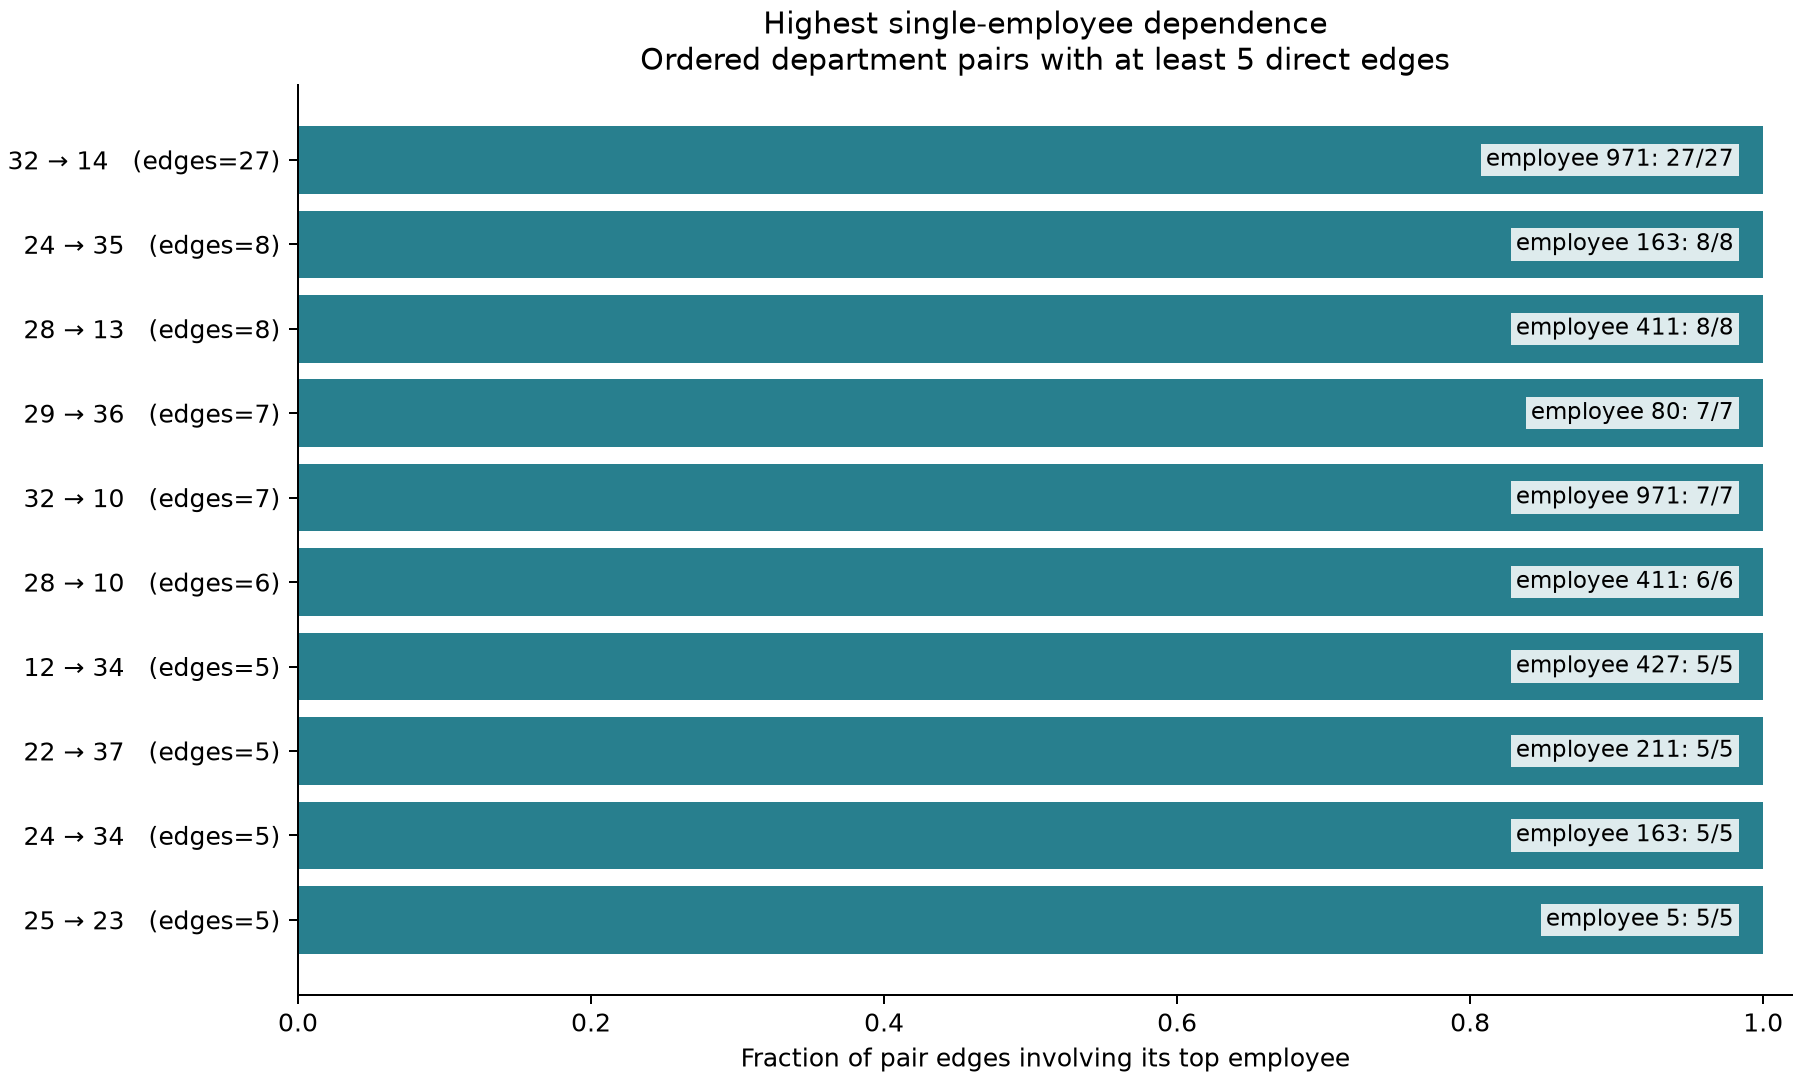
\includegraphics[width=0.92\linewidth]{figures/department_dependence.png}
\caption{Ten highest-dependence department pairs among those with edge support $|E_{AB}| \ge 5$. Department pair $32 \to 14$ exhibits complete dependence ($D_{AB} = 1.0$) across all 27 directed edges, concentrated entirely in employee 971.}
\label{fig:dept_dependence}
\end{figure}

\begin{figure}[htbp]
\centering
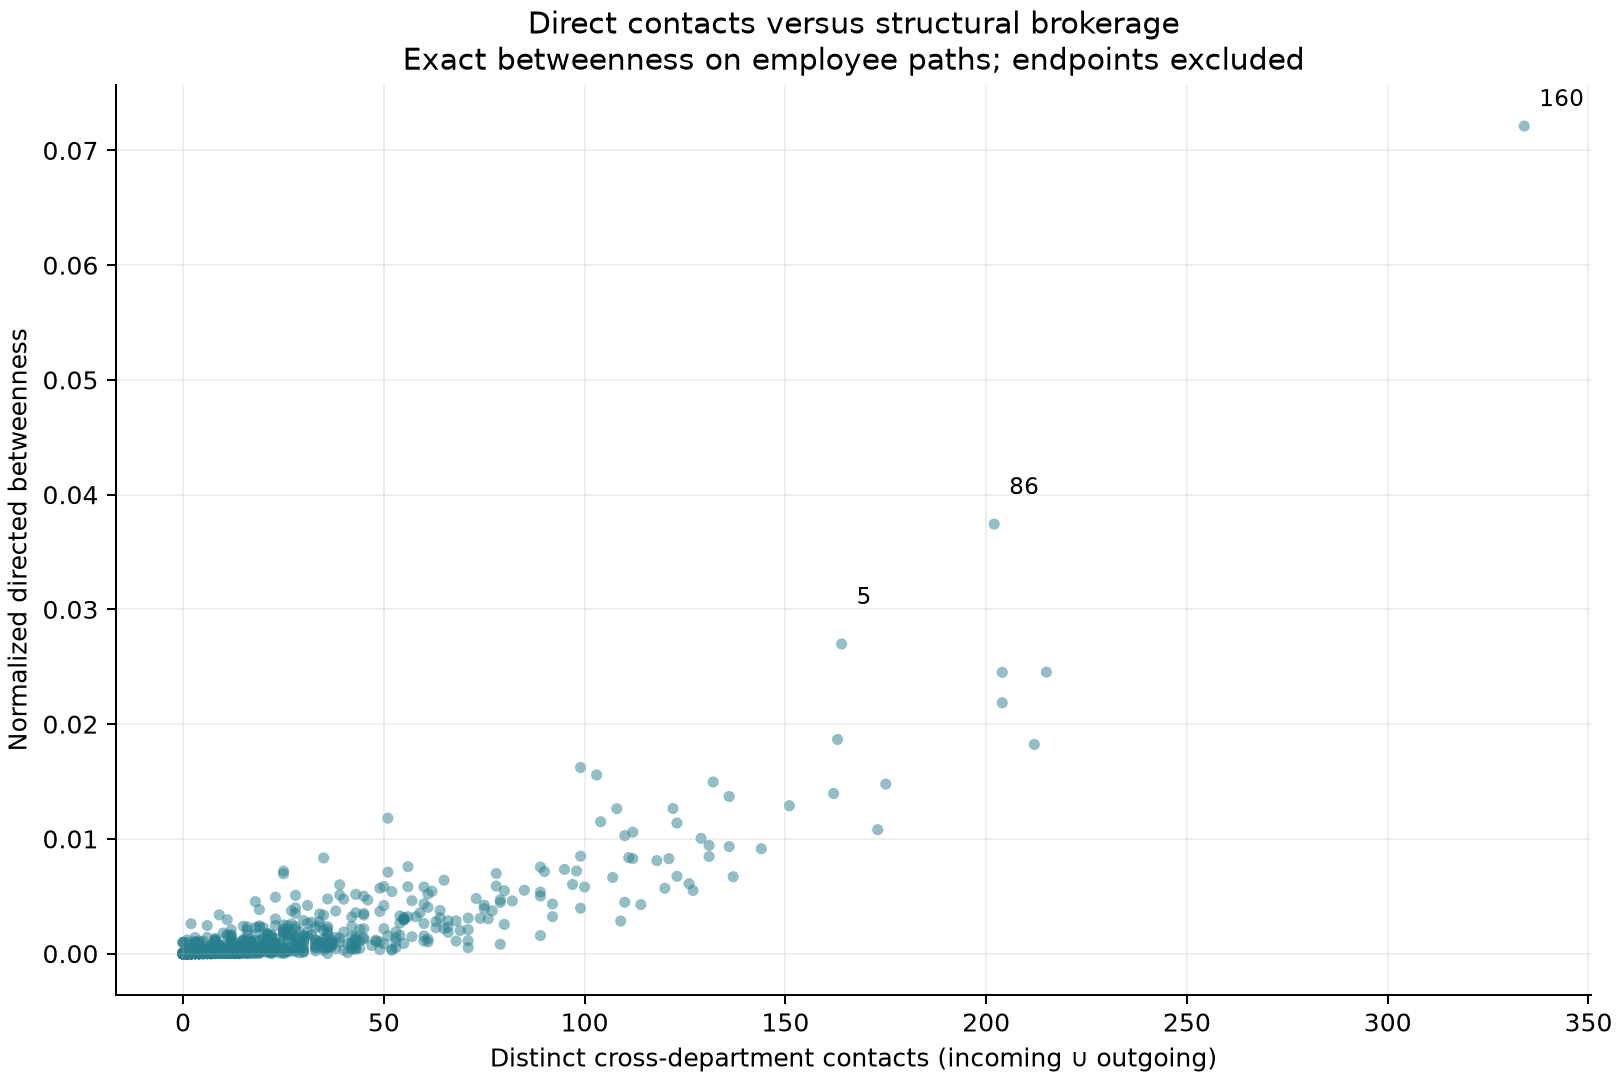
\includegraphics[width=0.92\linewidth]{figures/employee_rankings.png}
\caption{Cross-department contacts vs. exact normalized directed betweenness for all 1,005 employees. While top nodes correlate, substantial off-diagonal discordance demonstrates that local contact volume diverges from global path brokerage.}
\label{fig:employee_rankings}
\end{figure}

\begin{figure*}[htbp]
\centering
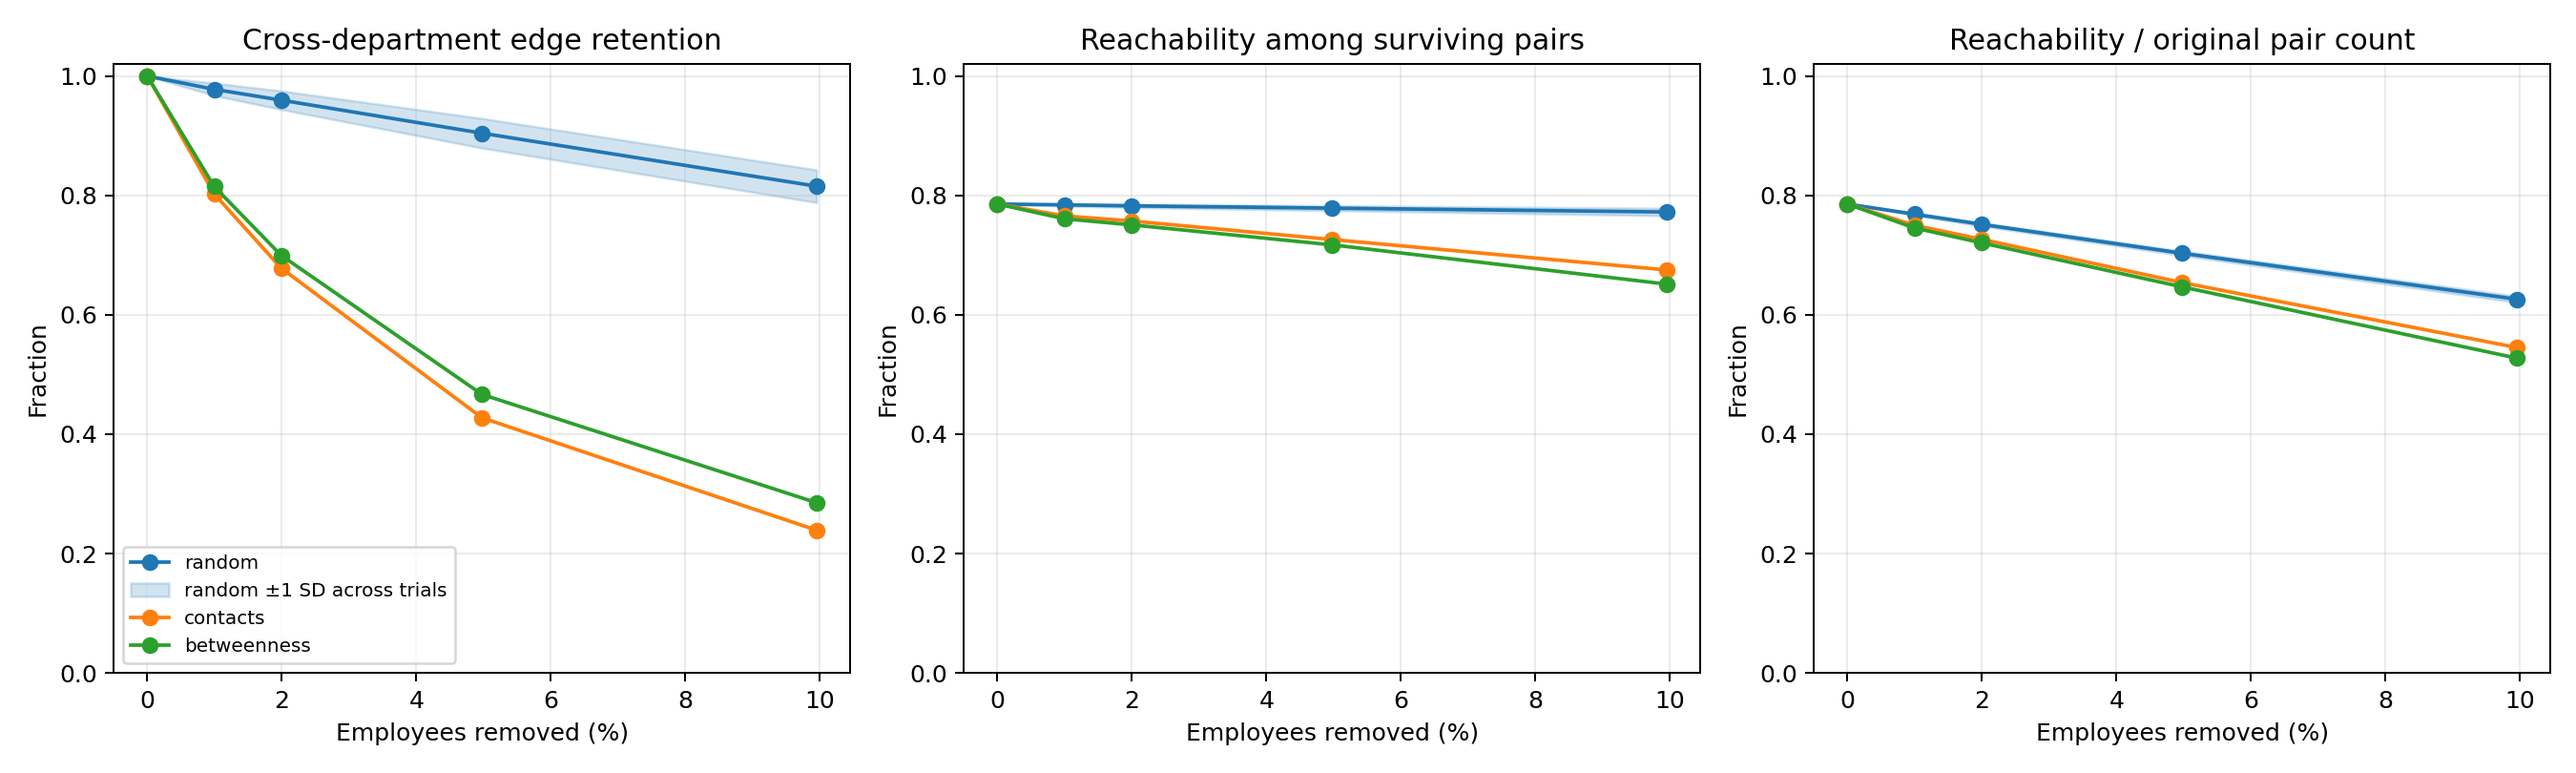
\includegraphics[width=0.98\linewidth]{figures/removal_comparison.png}
\caption{Comparative resilience under random, contact-targeted, and betweenness-targeted employee removal across 0\% to 10\% workforce removal budgets. (Left) Cross-department edge retention; (Center) Directed reachability among surviving pairs; (Right) Reachable pairs normalized by the initial pair count ($961,932$). Shaded bands indicate $\pm 1$ sample standard deviation across 30 random trials.}
\label{fig:removal_comparison}
\end{figure*}

\subsection{Preliminary Results}

\textbf{High pairwise dependence with substantial edge support.}
Among the $42 \times 41 = 1,722$ possible directed department pairs, $1,203$ pairs have at least one directed edge. The overall median dependence is $0.50$, and $308$ pairs exhibit $D_{AB} = 1.0$. As shown in Table~\ref{tab:dependence_thresholds}, filtering by minimum edge support confirms that high concentration is not merely an artifact of sparse single-edge pairs: $13$ pairs maintain $D_{AB} = 1.0$ at $|E_{AB}| \ge 5$. Notably, as shown in Fig.~\ref{fig:dept_dependence}, all $27$ directed edges from Department 32 to Department 14 involve a single individual (Employee 971), representing a critical institutional single-point vulnerability. Similarly, for Department $24 \to 36$, Employee 163 mediates 14 of 15 edges ($D_{AB} = 0.933$).

\begin{table}[htbp]
\caption{Department Dependence Under Support Thresholds}
\begin{center}
\footnotesize
\setlength{\tabcolsep}{3.5pt}
\begin{tabular}{cccc}
\toprule
\textbf{Support ($k$)} & \textbf{Pairs Retained} & \textbf{Pairs with $D_{AB}=1$} & \textbf{Median $D_{AB}$} \\
\midrule
$|E_{AB}| \ge 1$  & 1,203 & 308 & 0.500 \\
$|E_{AB}| \ge 5$  & 673   & 13  & 0.400 \\
$|E_{AB}| \ge 10$ & 450   & 1   & 0.364 \\
\bottomrule
\end{tabular}
\label{tab:dependence_thresholds}
\end{center}
\end{table}

\textbf{Divergence between contacts and path brokerage.}
As visualized in Fig.~\ref{fig:employee_rankings}, Employee 160 (Department 36) ranks first in both metrics, with $334$ cross-department contacts and normalized directed betweenness of $0.07212$. While the top-10 sets share 8 employees, notable discrepancies exist: Employee 377 ranks 9th in betweenness but only 42nd in contacts; Employee 129 ranks 10th in betweenness but 39th in contacts. This confirms that certain employees act as critical structural bridges despite having moderate local degree.

\begin{table}[htbp]
\caption{Resilience Metrics at 100 Employees Removed (9.95\% Workforce)}
\begin{center}
\footnotesize
\setlength{\tabcolsep}{3.5pt}
\begin{tabular}{lccc}
\toprule
\textbf{Strategy} & \textbf{Edge Ret.} & \textbf{Surv. Reach.} & \textbf{Orig. Reach.} \\
\midrule
Random (30 trials)   & 81.54\% & 77.22\% & 62.61\% \\
Contact-Targeted     & 23.91\% & 67.51\% & 54.52\% \\
Betweenness-Targeted & 28.51\% & 65.14\% & 52.74\% \\
\bottomrule
\end{tabular}
\label{tab:removal_results}
\end{center}
\end{table}

\textbf{Resilience under node removal.}
Table~\ref{tab:removal_results} and Fig.~\ref{fig:removal_comparison} summarize the node removal experiments. At $B=100$ (9.95\% workforce removed):
\begin{itemize}
    \item Random removal exhibits remarkable structural stability, retaining $81.54\%$ of cross-department edges and leaving $77.22\%$ survivor reachability ($62.61\%$ of initial pairs).
    \item Contact-targeted removal inflicts catastrophic edge attrition, preserving only $23.91\%$ of cross-department edges.
    \item Betweenness-targeted removal is significantly more lethal to directed path connectivity, driving survivor reachability down to $65.14\%$ ($52.74\%$ of initial pairs), despite preserving more raw edges ($28.51\%$) than contact-targeted removal.
\end{itemize}

\subsection{Significance and Discussion}
These preliminary results provide crucial insights into organizational network mechanics. First, they demonstrate that direct degree and shortest-path centrality target complementary structural layers: degree targeting rapidly strips local connectivity, whereas betweenness targeting dismantles global path efficiency. Second, despite the loss of over $76\%$ of direct cross-department edges under contact removal, more than $67\%$ of surviving employee pairs remain mutually reachable. This indicates high latent topological redundancy—information can reroute through secondary department bridges even when primary channels collapse.

\section{Conclusion and Short-Term Plans}

\subsection{Summary of Main Findings}
In this milestone, we characterized the department-level dependence and resilience of the SNAP email-Eu-core network. We demonstrated that inter-departmental communication is highly concentrated in specific bridge personnel, including cases where entire inter-departmental relationships rely on a single employee. Furthermore, our deletion experiments proved that betweenness-targeted departures degrade directed path reachability substantially faster than random or degree-based attrition.

\subsection{Plans for Milestone 2 and Final Presentations}
For the final milestone and presentation, our short-term technical roadmap includes:
\begin{enumerate}
    \item \textbf{Dynamic Adaptive Reranking:} Recomputing centralities dynamically after each deletion increment to model adaptive network degradation.
    \item \textbf{Resilience-Enhancing Interventions:} Designing and benchmarking targeted edge-addition algorithms (e.g., creating backup bridges between highly dependent department pairs) under fixed edge budgets to mitigate identified structural risks.
    \item \textbf{Null Model Comparison:} Benchmarking observed resilience metrics against synthetic degree-preserving configuration models to determine whether observed resilience stems from modular organizational hierarchy or generic degree distributions.
\end{enumerate}

\subsection{Individual Member Contributions}
\textbf{Jiening Yang:} Led the upstream structural analysis. Implemented data ingestion, network sanitization, descriptive graph metrics, exact pairwise departmental dependence formulation ($D_{AB}$), exact directed betweenness computations, employee ranking pipelines, and visualization figures (heatmap, dependence distribution, and ranking scatterplots). Prepared upstream documentation and initial slides.

\textbf{Yikang Cheng:} Led the downstream removal and resilience analysis. Designed and implemented the node-removal simulation framework, developed the exact directed reachability engine using SCC condensation DAGs, conducted Monte Carlo random trials, benchmarked edge retention against pair reachability, created comparative resilience figures, and implemented automated unit tests.

\begin{thebibliography}{00}
\bibitem{snap-email}
Stanford Network Analysis Project (SNAP), ``email-Eu-core network,'' \url{https://snap.stanford.edu/data/email-Eu-core.html}, accessed Oct. 2026.

\bibitem{yin2017local}
H.~Yin, A.~R.~Benson, J.~Leskovec, and D.~F.~Gleich, ``Local higher-order graph clustering,'' in \textit{Proc. 23rd ACM SIGKDD Int. Conf. Knowledge Discovery and Data Mining (KDD)}, 2017, pp. 555--564.

\bibitem{brandes2001faster}
U.~Brandes, ``A faster algorithm for betweenness centrality,'' \textit{Journal of Mathematical Sociology}, vol. 25, no. 2, pp. 163--177, 2001.

\bibitem{albert2000error}
R.~Albert, H.~Jeong, and A.-L.~Barab{\'a}si, ``Error and attack tolerance of complex networks,'' \textit{Nature}, vol. 406, no. 6794, pp. 378--382, 2000.

\bibitem{networkx-betweenness}
A.~A.~Hagberg, D.~A.~Schult, and P.~J.~Swart, ``Exploring network structure, dynamics, and function using NetworkX,'' in \textit{Proc. 7th Python in Science Conf. (SciPy)}, 2008, pp. 11--15.
\end{thebibliography}

\end{document}
